\section{Design and Implementation}
\label{arch}

VDMS implements a client-server design.
The VDMS Server handles client requests concurrently and coordinates
request execution across the metadata and data components in order to return a
unified response. The metadata component is the Persistent Memory Graph
Database (PMGD). The data component is our custom library, the
Visual Compute Library (VCL). The VCL enables machine friendly enhancements to
visual data.
VDMS and its components are fully available as open source tools
\footnote{https://github.com/IntelLabs/\{vdms, pmgd, vcl\}}.

\textbf{Persistent Memory Graph Database:}
Recent developments in persistent memory technologies
like 3D XPoint~\cite{IntelXPoint15}
promise storage elements  providing  nearly  the  speed  of  DRAM  and  the
durability of block-oriented storage. To provide an efficient storage
solution addressing the increasing popularity of connected data and
applications that benefit from graph like processing, we have designed
and implemented an in-persistent-memory graph database, PMGD, optimized
to run on a platform equipped with persistent memory.
PMGD provides a property graph model of data storage with the traditional
atomicity, consistency, isolation, and durability properties expected from
databases. The graph model makes it very suitable for the data model and
access patterns shown by visual metadata.
With its natural ability to extend the schema very
easily (due to the use of a property graph model),
we can support new developments in machine learning that can lead to
enhancements to existing metadata over time.
The specific details on how the data structures are optimized for persistent
memory, and the performance comparison with other graph databases is on-going
work that will be publish separately.

\textbf{Visual Compute Library:} The VCL was designed to provide an interface
through which users can interact with visual data. For traditional formats,
the interface is an abstraction layer over OpenCV. However, it also provides a
way to use novel formats that are better suited for visual analytics: a novel,
array-based lossless image format. This format is built on the array data
manager TileDB~\cite{TileDB} and is well suited for images that are used in
visual analytics.
The VCL currently provides limited support for videos but we are enhancing
its capabilities as part of our future work.
Feature vector support is provided through an implementation based
on high-dimensional sparse arrays, also using TileDB, which contains both
storage and search functionality over feature vectors.
In addition, the VCL provides a wrapper
for another high-dimensional index implementation,
Facebook's Faiss~\cite{faiss}.

\begin{comment}

\begin{figure*}[t!]
\begin{subfigure}{.5\textwidth}
  \centering
  \includegraphics[width=.92\linewidth]{figures/query}
  \caption{Simple Metadata Query.}
  \label{fig:sfig1}
\end{subfigure}%
\begin{subfigure}{.52\textwidth}
  \centering
  \includegraphics[width=.94\linewidth]{figures/query2}
  \caption{Query involving visual transformations.}
  \label{fig:sfig2}
\end{subfigure}
\begin{subfigure}{\textwidth}
  \centering
  \includegraphics[width=.9\linewidth]{figures/results}
  \caption{Original image (left) and the result of query in (b)}
  \label{fig:sfig3}
\end{subfigure}
\caption{Snapshot of a Python notebook with sample queries}
\label{fig:query}
\end{figure*}

\end{comment}

\textbf{Request Server:}
Developers and users of machine learning frameworks and data science
applications favor simpler interfaces to access and process data and cannot
be expected to deal with two different ways of interacting with information (
metadata and visual data) instead of focusing on the algorithmic parts of their
pipelines.
VDMS takes care of coordinating client requests across the metadata and the
data as well as efficiently manages multiple clients through its Request
Server component, by implementing a JSON-based API.
It decomposes the command into
metadata and data requests, invokes the relevant calls behind the scene,
and returns a coherent response to the user after applying any additional
operations (explained in the next section).

% \textbf{Client Library:}
% A user application can use the VDMS API by defining metadata conforming to the
% query protocol we have defined and passing along blobs. The client side VDMS
% library provides a simple query function that accepts a JSON string with
% commands and an array or vector of blobs.
% Internally, the library wraps the query string and blob using Google Protobufs
% and sends it to VDMS. It also receives a similarly wrapped response from VDMS
% and returns it to the client. The responses require JSON parsing on the client
% side for the metadata string that indicates how to interpret blobs.
% VDMS provides Python and C++ client libraries with mainly
% one function: a query that passes metadata as a JSON string and,
% optionally, data as a vector of blobs. The VDMS client library manages the
% rest.

\section{VDMS API}
\label{arch}
One of our goals with VDMS was to define an API that is easy to use.
Our API explicitly predefines certain
visual primitives associated with images, videos, and feature vectors. In
addition, while we use a graph database to store our metadata, the API is not
graph specific.
We have paid particular attention to hide the complexities of our internal
implementation and up-level the API to a JSON-based
API\footnote{https://github.com/IntelLabs/vdms/wiki/API-Description},
which is very popular across various application domains.
We understand that by defining a new JSON-based API we had to trade-off
expressiveness (compared to SPARQL or Gremlim) for the ability to design
native support for visual data, but we believe that, as development of VDMS
evolves, we will be able to achieve similar levels of expressiveness compared
to more mature query languages.
We have developed Python and C++ client
library to provide a simple query function that accepts a JSON string with
commands and an array or vector of blobs.

\begin{comment} 
% All of the folliwng is commented out.

\begin{figure}[ht!]
\centering
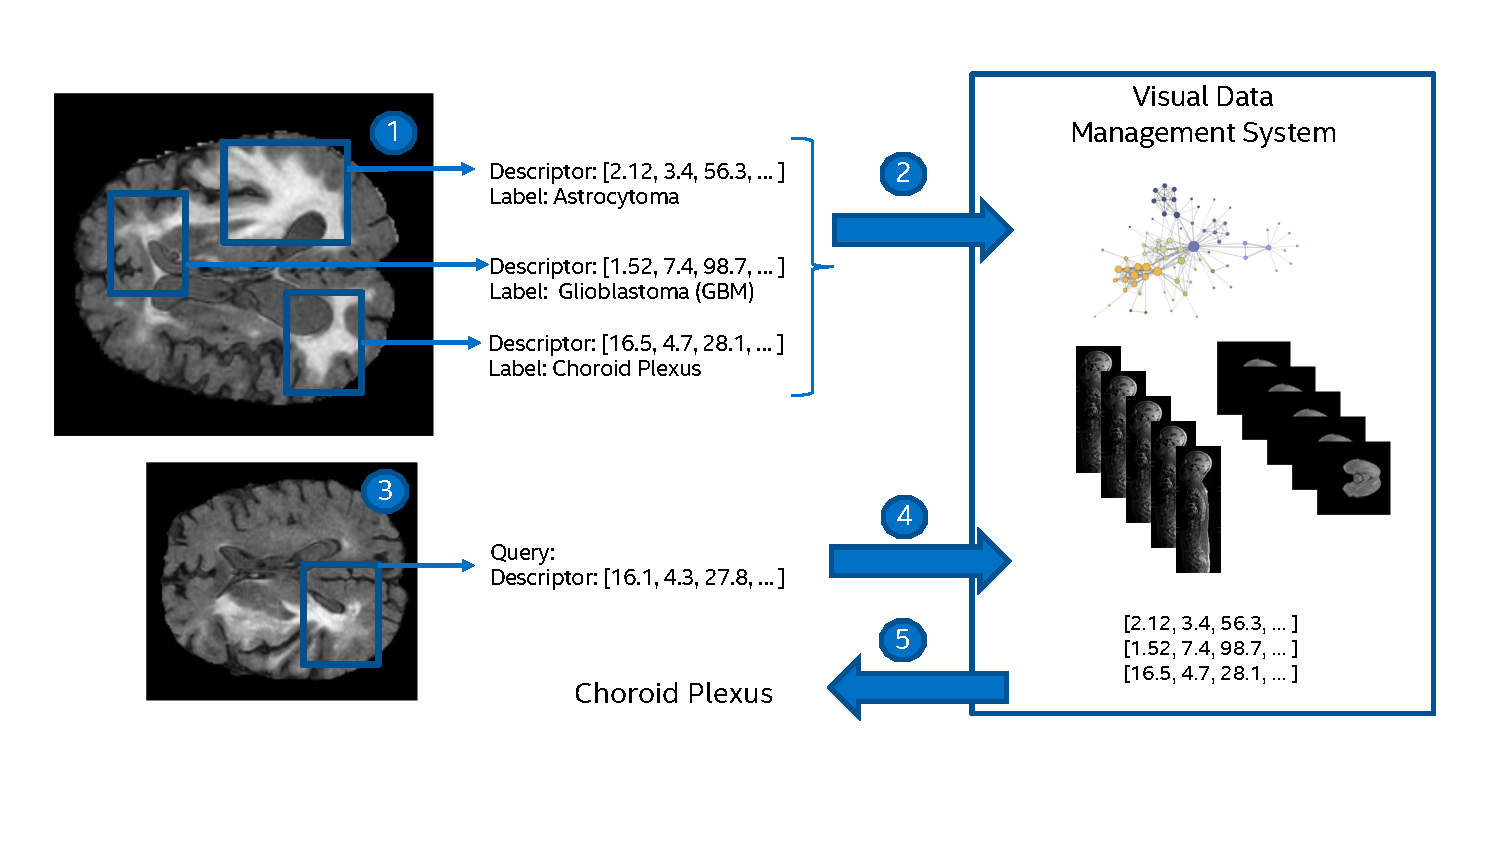
\includegraphics[width=0.9\columnwidth]{figures/features}
\caption{Feature Vectors natively supported in VDMS}
\label{fig:features}
\end{figure}

We use a medical imaging dataset as a driving example, and use it
here to showcase our API. More details about this use case are discussed in
Section~\ref{demo}.
Figure~\ref{fig:query} shows a snapshot from a Jupyter Notebook with two
simple queries.
Figure~\ref{fig:sfig1} shows a simple metadata query
where information about properties of patients matching some specific
characteristics (admitted with 85 years of age or more)
is used to constrain the search.
The returned JSON structure shows 2 patients found in the database.
Note that in this examples the queries are expressed as plain strings to
help the reader understand its structure. In real applications, the queries
are structured using the preferred method or library
for handling JSON structures (e.g. Python dictionaries or jsoncpp in C++).

Figure~\ref{fig:sfig2} shows a query involving visual transformations.
In this case, the query is looking for an image with a certain \textit{id}
value, and expects  VDMS to return the image twice: once with a thresholding
transformation (e.g., zero out all pixels less than a threshold), and the
second time after applying a threshold and then resizing it.
\ref{fig:sfig3} shows the image originally inserted in VDMS (left),
along with the returned images corresponding to the query in \ref{fig:sfig2}.
Adding new operations to VDMS is easy, as our software architecture
encapsulates all operations in VCL, and any new operation can use
or wrap around OpenCV, which is used internally.

\end{comment} 
% End of Comment


Another key differentiating factor of VDMS is that it allows the creation of
indexes for high-dimensional feature vectors and the insertion of
these feature vectors associated with entities or visual objects.
Feature vectors are intermediate results of various machine
learning or computer vision algorithms when run on visual data.
These vectors can be labeled and classified to build search indexes,
and there are many in-memory libraries that are designed for
this task~\cite{flann, faiss}.
Using the VDMS API, users can manage feature vector indexes,
query previously inserted elements (images),
run a k-nearest neighbor search (knn) and express relationships
between existing images or feature vectors and
the newly inserted feature vectors.
By natively supporting feature vectors and knn,
VDMS allows out-of-the-box classification
functionalities for many applications.
Figure~\ref{fig:features} shows an example of how this functionality
can be integrated in a medical imaging analytics pipeline:
(1) A feature vector is extracted from an bounding
box in a brain image and labeled;
(2) the feature vector is inserted together
with all the associated metadata (type of cancer, for example)
and a link to the original image.
(3) A new feature vector is extracted from a new image,
(4) a query to VDMS is issued to classify that feature vector based on the
indexed features in VDMS, and
(5) VDMS can respond to the query with the label
associated to that feature vector.
Note that, even if the example is based on the medical images used for the
performance evaluation, this methodology is applicable in many other contexts
and use cases, such as face detection and matching.
More details about the JSON API for this functionality can be found on
our Github wiki page.
